% Document/LinearAlgebra/VectorSpaces/Foundations/Span.tex
% Section: Span (Generated Subspaces)

\newpage
\section{Span}

\begin{definition}[Span]\label{def:span}
    Let $V$ be a $K$-vector space and $S \subseteq V$. The \textbf{span} (or \textbf{linear span})
    of $S$ is the smallest subspace of $V$ containing $S$:
    \[
        \Span[K]{S} = \BigIntersect \Set{U \Subspace[K] V \mid S \subseteq U}
    \]
\end{definition}

\begin{example}[Spans in Coordinate Spaces]\label{ex:span-examples}
    Consider the following examples:
    \begin{enumerate}
        \item $\Span[\bb{R}]{\{(1,0)\}} = $ the $x$-axis in $\bb{R}^2$
        \item $\Span[\bb{R}]{\{(1,0), (0,1)\}} = \bb{R}^2$
        \item $\Span[K]{\{1, X, X^2\}} = K[X]_{\leq 2}$ (polynomials of degree at most $2$)
    \end{enumerate}

    \begin{center}
    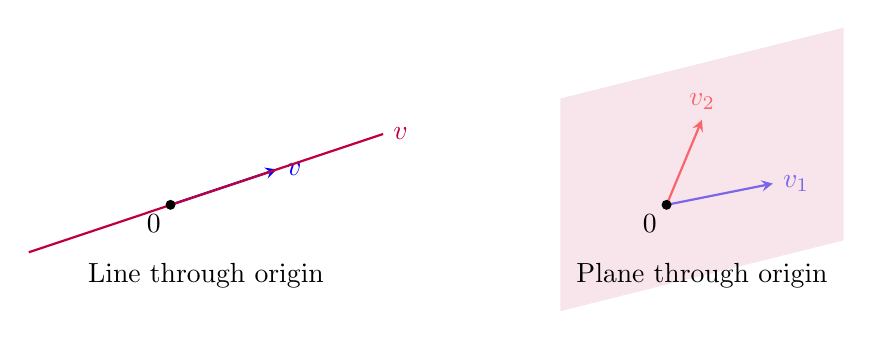
\begin{tikzpicture}[scale=0.9, >=stealth]
        % Span of one vector
        \begin{scope}
            \draw[->, thick, blue] (0,0) -- (1.5,0.5) node[right] {$v$};
            \draw[thick, purple] (-2,-0.67) -- (3,1) node[right] {$\Span{v}$};
            \fill (0,0) circle (2pt) node[below left] {$0$};
            \node at (0.5,-1) {Line through origin};
        \end{scope}

        % Span of two non-collinear vectors
        \begin{scope}[xshift=7cm]
            \draw[->, thick, blue] (0,0) -- (1.5,0.3) node[right] {$v_1$};
            \draw[->, thick, red] (0,0) -- (0.5,1.2) node[above] {$v_2$};
            \fill[purple!20, opacity=0.5] (-1.5,-1.5) -- (2.5,-0.5) -- (2.5,2.5) -- (-1.5,1.5) -- cycle;
            \fill (0,0) circle (2pt) node[below left] {$0$};
            \node at (0.5,-1) {Plane through origin};
        \end{scope}
    \end{tikzpicture}
    \end{center}
\end{example}

\begin{example}[Spans in $\bb{R}^3$]\label{ex:span-R3}
    In $\bb{R}^3$, consider the standard basis vectors $e_1 = (1,0,0)$, $e_2 = (0,1,0)$, $e_3 = (0,0,1)$:
    \begin{enumerate}
        \item \textbf{Line}: $\Span[\bb{R}]{\{e_3\}} = \Set{(0, 0, z) \mid z \in \bb{R}}$ (the $z$-axis)
        \item \textbf{Plane}: $\Span[\bb{R}]{\{e_1, e_2\}} = \Set{(x, y, 0) \mid x, y \in \bb{R}}$ (the $xy$-plane)
        \item \textbf{Whole space}: $\Span[\bb{R}]{\{e_1, e_2, e_3\}} = \bb{R}^3$
    \end{enumerate}

    \textbf{Non-example}: $\{(1, 0, 0), (2, 0, 0)\}$ spans only a line, not a plane, because $(2, 0, 0) = 2 \cdot (1, 0, 0)$ is redundant.

    \begin{center}
    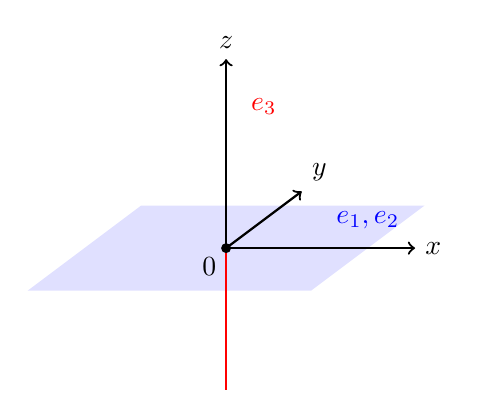
\begin{tikzpicture}[scale=1.2,
        x={(1cm,0cm)},
        y={(0.4cm,0.3cm)},
        z={(0cm,1cm)}]

        % xy-plane (span of e1, e2)
        \fill[blue!20, opacity=0.6] (-1.5,-1.5,0) -- (1.5,-1.5,0) -- (1.5,1.5,0) -- (-1.5,1.5,0) -- cycle;
        \node[blue] at (1.5, 0, 0.3) {$\Span{e_1, e_2}$};

        % z-axis (span of e3)
        \draw[thick, red] (0,0,-1.5) -- (0,0,1.5);
        \node[red] at (0.4,0,1.5) {$\Span{e_3}$};

        % Coordinate axes
        \draw[->, thick] (0,0,0) -- (2,0,0) node[right] {$x$};
        \draw[->, thick] (0,0,0) -- (0,2,0) node[above right] {$y$};
        \draw[->, thick] (0,0,0) -- (0,0,2) node[above] {$z$};

        % Origin
        \fill (0,0,0) circle (1.5pt) node[below left] {$0$};
    \end{tikzpicture}
    \end{center}
\end{example}


\begin{proposition}[Constructive Characterization of Span]\label{prop:span-constructive}
    For any $S \subseteq V$:
    \[
        \Span[K]{S} = \Set{\sum_{i=1}^{n} a_i v_i \mid n \in \bb{N}, a_i \in K, v_i \in S}
    \]
    That is, $\Span[K]{S}$ equals the set of all finite $K$-linear combinations of elements in $S$.
\end{proposition}

\begin{proof}
    Let $L$ denote the set of all finite linear combinations of elements in $S$.

    \textbf{($\Span[K]{S} \subseteq L$)}:
    We show $L$ is a subspace containing $S$, hence contains $\Span[K]{S}$.
    \begin{itemize}
        \item $L \neq \emptyset$: The empty sum gives $0 \in L$.
        \item \textbf{Closure}: If $x = \sum_{i=1}^{n} a_i v_i$ and $y = \sum_{j=1}^{m} b_j w_j$ are in $L$, then
              for $\alpha, \beta \in K$:
              \[
                  \alpha x + \beta y = \sum_{i=1}^{n} \alpha a_i v_i + \sum_{j=1}^{m} \beta b_j w_j \in L
              \]
        \item $S \subseteq L$: Each $v \in S$ equals $1 \cdot v \in L$.
    \end{itemize}
    By definition of span, $\Span[K]{S} \subseteq L$.

    \textbf{($L \subseteq \Span[K]{S}$)}:
    Let $U$ be any subspace with $S \subseteq U$. Every linear combination of elements in $S$
    lies in $U$ (by Proposition~\ref{prop:subspace-lincomb}), so $L \subseteq U$.
    Thus $L \subseteq \BigIntersect\Set{U : S \subseteq U} = \Span[K]{S}$.
\end{proof}

\begin{proposition}[Properties of Span]\label{prop:span-properties}
    The span operation satisfies:
    \begin{enumerate}
        \item $\Span[K]{S}$ is a subspace of $V$
        \item $S \subseteq \Span[K]{S}$
        \item If $S \subseteq U$ where $U \Subspace[K] V$, then $\Span[K]{S} \subseteq U$
        \item \textbf{Monotonicity}: $S \subseteq T \implies \Span[K]{S} \subseteq \Span[K]{T}$
        \item \textbf{Idempotence}: $\Span[K]{\Span[K]{S}} = \Span[K]{S}$
        \item \textbf{Subspace criterion}: $U$ is a subspace iff $\Span[K]{U} = U$
        \item \textbf{Union}: $\Span[K]{S \Union T} = \Span[K]{\Span[K]{S} \Union \Span[K]{T}}$
    \end{enumerate}
\end{proposition}

\begin{proof}
    (1) Follows from Proposition~\ref{prop:intersection-subspace}.

    (2) Each $v \in S$ is contained in every subspace containing $S$.

    (3) This is the definition: $\Span[K]{S}$ is the intersection of all such $U$.

    (4) If $S \subseteq T$, then every subspace containing $T$ also contains $S$,
    so $\Span[K]{S} \subseteq \Span[K]{T}$.

    (5) $\Span[K]{S}$ is a subspace containing itself, so $\Span[K]{\Span[K]{S}} \subseteq \Span[K]{S}$.
    By (2), $\Span[K]{S} \subseteq \Span[K]{\Span[K]{S}}$.

    (6) ($\Rightarrow$) If $U$ is a subspace, then $U$ is the smallest subspace containing $U$, so $\Span[K]{U} = U$.
    ($\Leftarrow$) If $\Span[K]{U} = U$, then $U$ is a subspace by (1).

    (7) By monotonicity, $\Span[K]{S} \Union \Span[K]{T} \subseteq \Span[K]{S \Union T}$, so
    $\Span[K]{\Span[K]{S} \Union \Span[K]{T}} \subseteq \Span[K]{S \Union T}$.
    Conversely, $S \Union T \subseteq \Span[K]{S} \Union \Span[K]{T}$, so
    $\Span[K]{S \Union T} \subseteq \Span[K]{\Span[K]{S} \Union \Span[K]{T}}$.
\end{proof}

\begin{corollary}[Span of Empty Set and Zero]\label{cor:span-empty-zero}
    The following hold:
    \begin{enumerate}
        \item $\Span[K]{\emptyset} = \{0\}$
        \item $\Span[K]{\{0\}} = \{0\}$
    \end{enumerate}
\end{corollary}

\begin{proof}
    (1) The only linear combination of elements from $\emptyset$ is the empty sum, which equals $0$.
    Thus $\Span[K]{\emptyset} = \{0\}$.

    (2) Every linear combination of $0$ has the form $\sum_{i=1}^n a_i \cdot 0 = 0$.
    Thus $\Span[K]{\{0\}} = \{0\}$.
\end{proof}

\begin{proposition}[Sum as Span]\label{prop:sum-as-span}
    For subspaces $U, W \Subspace[K] V$:
    \[
        U + W = \Span[K]{U \Union W}
    \]
\end{proposition}

\begin{proof}
    \textbf{($U + W \subseteq \Span[K]{U \Union W}$)}:
    Every element of $U + W$ has the form $u + w$ with $u \in U$, $w \in W$.
    This is a linear combination of elements in $U \Union W$, hence in $\Span[K]{U \Union W}$.

    \textbf{($\Span[K]{U \Union W} \subseteq U + W$)}:
    Since $U, W \subseteq U + W$ (take $w = 0$ or $u = 0$), we have $U \Union W \subseteq U + W$.
    Since $U + W$ is a subspace (Proposition~\ref{prop:minkowski-subspace}),
    $\Span[K]{U \Union W} \subseteq U + W$.
\end{proof}

\begin{proposition}[Arbitrary Sums as Span]\label{prop:arbitrary-sum-span}
    For a family $(U_i)_{i \in I}$ of subspaces:
    \[
        \SubspaceSum{i \in I}{U_i} = \Span[K]{\BigUnion[i \in I] U_i}
    \]
\end{proposition}

\begin{proof}
    Let $S = \SubspaceSum{i \in I}{U_i}$ denote the subspace sum.
    
    \textbf{($S \subseteq \Span[K]{\BigUnion[i \in I] U_i}$)}:
    Every element of $S$ has the form $\sum_{j \in F} u_j$ where $F \subseteq I$ is finite
    and $u_j \in U_j$ for each $j \in F$. Since each $u_j \in U_j \subseteq \BigUnion[i \in I] U_i$,
    this is a finite linear combination (with coefficients $1$) of elements in $\BigUnion[i \in I] U_i$.
    Hence $\sum_{j \in F} u_j \in \Span[K]{\BigUnion[i \in I] U_i}$.
    
    \textbf{($\Span[K]{\BigUnion[i \in I] U_i} \subseteq S$)}:
    First, $\BigUnion[i \in I] U_i \subseteq S$: for any $u \in U_j$, we have $u = \sum_{i \in \{j\}} u$
    where $\{j\}$ is a finite subset of $I$ and $u \in U_j$, so $u \in S$.
    
    Since $S$ is a subspace (Proposition~\ref{prop:sum-subspace}) containing $\BigUnion[i \in I] U_i$,
    by the minimality of span, $\Span[K]{\BigUnion[i \in I] U_i} \subseteq S$.
\end{proof}

\begin{proposition}[Sum of Spans]\label{prop:sum-of-spans}
    For a family $(S_i)_{i \in I}$ of subsets of $V$:
    \[
        \SubspaceSum{i \in I}{\Span[K]{S_i}} = \Span[K]{\BigUnion[i \in I] S_i}
    \]
\end{proposition}

\begin{proof}
    By Proposition~\ref{prop:arbitrary-sum-span}:
    \[
        \SubspaceSum{i \in I}{\Span[K]{S_i}} = \Span[K]{\BigUnion[i \in I] \Span[K]{S_i}}
    \]
    Since $S_i \subseteq \Span[K]{S_i}$, we have $\BigUnion[i] S_i \subseteq \BigUnion[i] \Span[K]{S_i}$.
    Each $\Span[K]{S_i} \subseteq \Span[K]{\BigUnion[j] S_j}$ by monotonicity, so
    $\BigUnion[i] \Span[K]{S_i} \subseteq \Span[K]{\BigUnion[j] S_j}$.

    By idempotence:
    \[
        \Span[K]{\BigUnion[i] \Span[K]{S_i}} = \Span[K]{\BigUnion[i] S_i}
    \]
\end{proof}

\begin{definition}[Generating System]\label{def:generating-system}
    A subset $G \subseteq V$ is a \textbf{generating system} (or \textbf{spanning set}) for $V$
    if $\Span[K]{G} = V$.
\end{definition}

\begin{example}[Generating Systems]\label{ex:generating}
    Consider the following examples:
    \begin{enumerate}
        \item $\{(1, 0), (0, 1)\}$ generates $\bb{R}^2$ (standard basis)
        \item $\{(1, 0), (0, 1), (1, 1)\}$ also generates $\bb{R}^2$ (redundant generator)
        \item $\{1, X, X^2, \ldots\}$ generates $K[X]$
        \item Every vector space has a generating system: $V = \Span[K]{V}$
    \end{enumerate}
\end{example}

\begin{proposition}[$V$ Generates $V$]\label{prop:V-generates-V}
    Every vector space $V$ is a generating system for itself: $\Span[K]{V} = V$.
\end{proposition}

\begin{proof}
    Since $V$ is a subspace containing $V$, we have $\Span[K]{V} \subseteq V$.
    By Proposition~\ref{prop:span-properties}(2), $V \subseteq \Span[K]{V}$.
    Hence $\Span[K]{V} = V$.
\end{proof}

\begin{proposition}[Superset of Generating is Generating]\label{prop:superset-generating}
    If $G$ generates $V$ and $G \subseteq H \subseteq V$, then $H$ generates $V$.
\end{proposition}

\begin{proof}
    By monotonicity: $V = \Span[K]{G} \subseteq \Span[K]{H} \subseteq V$.
\end{proof}
